\documentclass{standalone}
\usepackage{tikz}
\usetikzlibrary{patterns, positioning}


\begin{document}
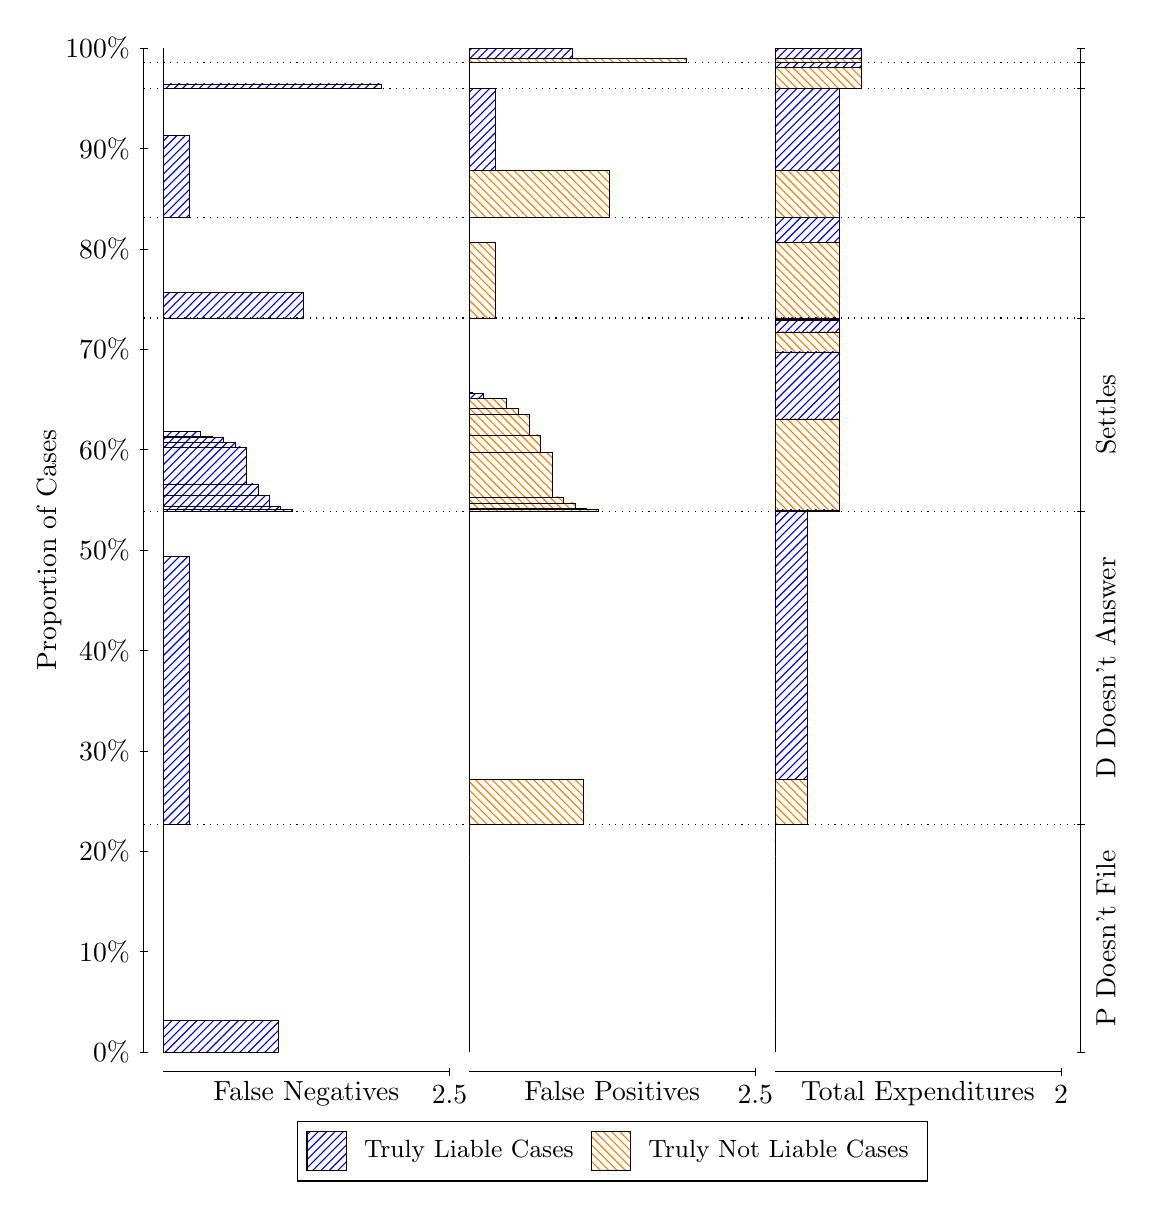
\begin{tikzpicture}
\draw[black, very thin] (1.5,1.75) -- (1.5,14.5);
\node[rotate=90, text=black, anchor=center] at (0.3, 8.125) {Proportion of Cases};
\draw[black, very thin] (1.45,1.75) -- (1.55,1.75);
\node[text=black, anchor=east] at (1.45, 1.75) {0\%};
\draw[black, very thin] (1.45,3.025) -- (1.55,3.025);
\node[text=black, anchor=east] at (1.45, 3.025) {10\%};
\draw[black, very thin] (1.45,4.3) -- (1.55,4.3);
\node[text=black, anchor=east] at (1.45, 4.3) {20\%};
\draw[black, very thin] (1.45,5.575) -- (1.55,5.575);
\node[text=black, anchor=east] at (1.45, 5.575) {30\%};
\draw[black, very thin] (1.45,6.85) -- (1.55,6.85);
\node[text=black, anchor=east] at (1.45, 6.85) {40\%};
\draw[black, very thin] (1.45,8.125) -- (1.55,8.125);
\node[text=black, anchor=east] at (1.45, 8.125) {50\%};
\draw[black, very thin] (1.45,9.4) -- (1.55,9.4);
\node[text=black, anchor=east] at (1.45, 9.4) {60\%};
\draw[black, very thin] (1.45,10.675) -- (1.55,10.675);
\node[text=black, anchor=east] at (1.45, 10.675) {70\%};
\draw[black, very thin] (1.45,11.95) -- (1.55,11.95);
\node[text=black, anchor=east] at (1.45, 11.95) {80\%};
\draw[black, very thin] (1.45,13.225) -- (1.55,13.225);
\node[text=black, anchor=east] at (1.45, 13.225) {90\%};
\draw[black, very thin] (1.45,14.5) -- (1.55,14.5);
\node[text=black, anchor=east] at (1.45, 14.5) {100\%};

\draw[black, very thin] (13.4,1.75) -- (13.4,14.5);
\draw[black, very thin] (13.35,1.75) -- (13.45,1.75);
\node[anchor=west] at (13.35, 1.75) {};
\draw[black, very thin] (13.35,4.6379) -- (13.45,4.6379);
\node[anchor=west] at (13.35, 4.6379) {};
\draw[black, very thin] (13.35,8.6141) -- (13.45,8.6141);
\node[anchor=west] at (13.35, 8.6141) {};
\draw[black, very thin] (13.35,11.072) -- (13.45,11.072);
\node[anchor=west] at (13.35, 11.072) {};
\draw[black, very thin] (13.35,12.352) -- (13.45,12.352);
\node[anchor=west] at (13.35, 12.352) {};
\draw[black, very thin] (13.35,13.989) -- (13.45,13.989);
\node[anchor=west] at (13.35, 13.989) {};
\draw[black, very thin] (13.35,14.313) -- (13.45,14.313);
\node[anchor=west] at (13.35, 14.313) {};
\draw[black, very thin] (13.35,14.5) -- (13.45,14.5);
\node[anchor=west] at (13.35, 14.5) {};

\draw[black, very thin, pattern color=blue, pattern=north east lines] (1.75,1.75) rectangle (3.2033,2.1546);
\draw[black, very thin, pattern color=orange, pattern=north west lines] (1.75,2.1546) rectangle (1.75,4.6379);
\draw[black, very thin, pattern color=blue, pattern=north east lines] (1.75,4.6379) rectangle (2.077,8.0391);
\draw[black, very thin, pattern color=orange, pattern=north west lines] (1.75,8.0391) rectangle (1.75,8.6141);
\draw[black, very thin, pattern color=blue, pattern=north east lines] (1.75,8.6141) rectangle (3.385,8.6392);
\draw[black, very thin, pattern color=blue, pattern=north east lines] (1.75,8.6392) rectangle (3.2397,8.6745);
\draw[black, very thin, pattern color=blue, pattern=north east lines] (1.75,8.6745) rectangle (3.0943,8.8174);
\draw[black, very thin, pattern color=blue, pattern=north east lines] (1.75,8.8174) rectangle (2.949,8.966);
\draw[black, very thin, pattern color=blue, pattern=north east lines] (1.75,8.966) rectangle (2.8037,9.4355);
\draw[black, very thin, pattern color=blue, pattern=north east lines] (1.75,9.4355) rectangle (2.6583,9.4914);
\draw[black, very thin, pattern color=blue, pattern=north east lines] (1.75,9.4914) rectangle (2.513,9.5529);
\draw[black, very thin, pattern color=blue, pattern=north east lines] (1.75,9.5529) rectangle (2.3677,9.5719);
\draw[black, very thin, pattern color=blue, pattern=north east lines] (1.75,9.5719) rectangle (2.2223,9.6323);
\draw[black, very thin, pattern color=orange, pattern=north west lines] (1.75,9.6323) rectangle (1.75,11.072);
\draw[black, very thin, pattern color=blue, pattern=north east lines] (1.75,11.072) rectangle (3.5303,11.394);
\draw[black, very thin, pattern color=orange, pattern=north west lines] (1.75,11.394) rectangle (1.75,12.352);
\draw[black, very thin, pattern color=blue, pattern=north east lines] (1.75,12.352) rectangle (2.077,13.393);
\draw[black, very thin, pattern color=orange, pattern=north west lines] (1.75,13.393) rectangle (1.75,13.989);
\draw[black, very thin, pattern color=blue, pattern=north east lines] (1.75,13.989) rectangle (4.5113,14.045);
\draw[black, very thin, pattern color=orange, pattern=north west lines] (1.75,14.045) rectangle (1.75,14.313);
\draw[black, very thin, pattern color=orange, pattern=north west lines] (1.75,14.313) rectangle (1.75,14.368);
\draw[black, very thin, pattern color=blue, pattern=north east lines] (1.75,14.368) rectangle (1.75,14.5);
\draw[black, very thin, pattern color=orange, pattern=north west lines] (5.6333,1.75) rectangle (5.6333,4.2332);
\draw[black, very thin, pattern color=blue, pattern=north east lines] (5.6333,4.2332) rectangle (5.6333,4.6379);
\draw[black, very thin, pattern color=orange, pattern=north west lines] (5.6333,4.6379) rectangle (7.0867,5.2128);
\draw[black, very thin, pattern color=blue, pattern=north east lines] (5.6333,5.2128) rectangle (5.6333,8.6141);
\draw[black, very thin, pattern color=orange, pattern=north west lines] (5.6333,8.6141) rectangle (7.2683,8.6365);
\draw[black, very thin, pattern color=orange, pattern=north west lines] (5.6333,8.6365) rectangle (7.123,8.6515);
\draw[black, very thin, pattern color=orange, pattern=north west lines] (5.6333,8.6515) rectangle (6.9777,8.7221);
\draw[black, very thin, pattern color=orange, pattern=north west lines] (5.6333,8.7221) rectangle (6.8323,8.8006);
\draw[black, very thin, pattern color=orange, pattern=north west lines] (5.6333,8.8006) rectangle (6.687,9.3648);
\draw[black, very thin, pattern color=orange, pattern=north west lines] (5.6333,9.3648) rectangle (6.5417,9.5875);
\draw[black, very thin, pattern color=orange, pattern=north west lines] (5.6333,9.5875) rectangle (6.3963,9.843);
\draw[black, very thin, pattern color=orange, pattern=north west lines] (5.6333,9.843) rectangle (6.251,9.9218);
\draw[black, very thin, pattern color=orange, pattern=north west lines] (5.6333,9.9218) rectangle (6.1057,10.054);
\draw[black, very thin, pattern color=blue, pattern=north east lines] (5.6333,10.054) rectangle (5.815,10.115);
\draw[black, very thin, pattern color=blue, pattern=north east lines] (5.6333,10.115) rectangle (5.6697,10.134);
\draw[black, very thin, pattern color=blue, pattern=north east lines] (5.6333,10.134) rectangle (5.6333,11.072);
\draw[black, very thin, pattern color=orange, pattern=north west lines] (5.6333,11.072) rectangle (5.9603,12.03);
\draw[black, very thin, pattern color=blue, pattern=north east lines] (5.6333,12.03) rectangle (5.6333,12.352);
\draw[black, very thin, pattern color=orange, pattern=north west lines] (5.6333,12.352) rectangle (7.4137,12.948);
\draw[black, very thin, pattern color=blue, pattern=north east lines] (5.6333,12.948) rectangle (5.9603,13.989);
\draw[black, very thin, pattern color=orange, pattern=north west lines] (5.6333,13.989) rectangle (5.6333,14.257);
\draw[black, very thin, pattern color=blue, pattern=north east lines] (5.6333,14.257) rectangle (5.6333,14.313);
\draw[black, very thin, pattern color=orange, pattern=north west lines] (5.6333,14.313) rectangle (8.3947,14.368);
\draw[black, very thin, pattern color=blue, pattern=north east lines] (5.6333,14.368) rectangle (6.9413,14.5);
\draw[black, very thin, pattern color=orange, pattern=north west lines] (9.5167,1.75) rectangle (9.5167,4.2332);
\draw[black, very thin, pattern color=blue, pattern=north east lines] (9.5167,4.2332) rectangle (9.5167,4.6379);
\draw[black, very thin, pattern color=orange, pattern=north west lines] (9.5167,4.6379) rectangle (9.9254,5.2128);
\draw[black, very thin, pattern color=blue, pattern=north east lines] (9.5167,5.2128) rectangle (9.9254,8.6141);
\draw[black, very thin, pattern color=orange, pattern=north west lines] (9.5167,8.6141) rectangle (10.334,8.6273);
\draw[black, very thin, pattern color=blue, pattern=north east lines] (9.5167,8.6273) rectangle (10.334,8.6352);
\draw[black, very thin, pattern color=orange, pattern=north west lines] (9.5167,8.6352) rectangle (10.334,9.7915);
\draw[black, very thin, pattern color=blue, pattern=north east lines] (9.5167,9.7915) rectangle (10.334,10.64);
\draw[black, very thin, pattern color=orange, pattern=north west lines] (9.5167,10.64) rectangle (10.334,10.895);
\draw[black, very thin, pattern color=blue, pattern=north east lines] (9.5167,10.895) rectangle (10.334,11.038);
\draw[black, very thin, pattern color=orange, pattern=north west lines] (9.5167,11.038) rectangle (10.334,11.053);
\draw[black, very thin, pattern color=blue, pattern=north east lines] (9.5167,11.053) rectangle (10.334,11.072);
\draw[black, very thin, pattern color=orange, pattern=north west lines] (9.5167,11.072) rectangle (10.334,12.03);
\draw[black, very thin, pattern color=blue, pattern=north east lines] (9.5167,12.03) rectangle (10.334,12.352);
\draw[black, very thin, pattern color=orange, pattern=north west lines] (9.5167,12.352) rectangle (10.334,12.948);
\draw[black, very thin, pattern color=blue, pattern=north east lines] (9.5167,12.948) rectangle (10.334,13.989);
\draw[black, very thin, pattern color=orange, pattern=north west lines] (9.5167,13.989) rectangle (10.607,14.257);
\draw[black, very thin, pattern color=blue, pattern=north east lines] (9.5167,14.257) rectangle (10.607,14.313);
\draw[black, very thin, pattern color=orange, pattern=north west lines] (9.5167,14.313) rectangle (10.607,14.368);
\draw[black, very thin, pattern color=blue, pattern=north east lines] (9.5167,14.368) rectangle (10.607,14.5);
\draw[black, dotted] (1.5,4.6379) -- (13.4,4.6379);
\draw[black, dotted] (1.5,8.6141) -- (13.4,8.6141);
\draw[black, dotted] (1.5,11.072) -- (13.4,11.072);
\draw[black, dotted] (1.5,12.352) -- (13.4,12.352);
\draw[black, dotted] (1.5,13.989) -- (13.4,13.989);
\draw[black, dotted] (1.5,14.313) -- (13.4,14.313);
\draw[black, very thin] (1.75,1.5) -- (5.3833,1.5);
\node[text=black, anchor=north] at (3.5667, 1.5) {False Negatives};
\draw[black, very thin] (5.3833,1.45) -- (5.3833,1.55);
\node[text=black, anchor=north] at (5.3833, 1.45) {2.5};

\draw[black, very thin] (5.6333,1.5) -- (9.2667,1.5);
\node[text=black, anchor=north] at (7.45, 1.5) {False Positives};
\draw[black, very thin] (9.2667,1.45) -- (9.2667,1.55);
\node[text=black, anchor=north] at (9.2667, 1.45) {2.5};

\draw[black, very thin] (9.5167,1.5) -- (13.15,1.5);
\node[text=black, anchor=north] at (11.333, 1.5) {Total Expenditures};
\draw[black, very thin] (13.15,1.45) -- (13.15,1.55);
\node[text=black, anchor=north] at (13.15, 1.45) {2};

\node[text=black, centered, rotate=90] at (13.72, 3.1939) {P Doesn't File};
\node[text=black, centered, rotate=90] at (13.72, 6.626) {D Doesn't Answer};
\node[text=black, centered, rotate=90] at (13.72, 9.8432) {Settles};





\draw (7.449999999999999,1.5) node[draw=none] (baseCoordinate) {};
\begin{scope}[align=center]
        \matrix[scale=0.5, draw=black, below=0.5cm of baseCoordinate, nodes={draw}, column sep=0.1cm]{
            \node[rectangle, draw, minimum width=0.5cm, minimum height=0.5cm, pattern color=blue, pattern=north east lines] {}; &
            \node[draw=none, font=\small, text=black] (B) {Truly Liable Cases}; &
            \node[rectangle, draw, minimum width=0.5cm, minimum height=0.5cm, pattern color=orange, pattern=north west lines] {}; &
            \node[draw=none, font=\small, text=black] (B) {Truly Not Liable Cases}; \\
            };
\end{scope}

\end{tikzpicture}
\end{document}